\documentclass[t]{beamer}
\usepackage[utf8]{inputenc} % to be able to type unicode text directly
\usepackage{inconsolata} % for a nicer (e.g. non-courier) tt family font

\usepackage{graphicx} % to include figures
\usepackage{hyperref,url} % to make clickable hyperlinks
\usepackage{minted} % for code insets
\usepackage{array} % to fine-tune tabular spacing
%\usepackage{graphbox} % to fine-tune image alignment
\usepackage{bbm} % for blackboard 1
\usepackage{soul} % for colored strikethrough

\colorlet{darkgreen}{black!50!green} % used for page numbers
\definecolor{term}{rgb}{.9,.9,.9} % used for code insets
\colorlet{darkred}{black!50!red}
\colorlet{lightgray}{black!50!gray}

\newcommand{\reference}[1] {{\scriptsize \color{gray}  #1 }}
\newcommand{\referencep}[1] {{\tiny \color{gray}  #1 }}
\newcommand{\unit}[1] {{\tiny \color{gray}  #1 }}

% coco's macros
\def\R{\mathbf{R}}
\def\F{\mathcal{F}}
\def\x{\mathbf{x}}
\def\u{\mathbf{u}}

%% disable spacing around verbatim
%\usepackage{etoolbox}
%\makeatletter
%\preto{\@verbatim}{\topsep=0pt \partopsep=0pt }
%\makeatother

% disable headings, set slide numbers in green
\mode<presentation>
\setbeamercolor*{author in head/foot}{parent=none}
\setbeamercolor*{title in head/foot}{parent=none}
\setbeamercolor*{date in head/foot}{parent=none}
\defbeamertemplate*{footline}{infoline theme}
{
  \leavevmode%
  \hfill\color{darkgreen}
   \insertframenumber{} / \inserttotalframenumber\hspace*{2ex}
  \vskip0pt%
}

% select red color for strikethrough
\makeatletter
\newcommand\SoulColor{%
  \let\set@color\beamerorig@set@color
  \let\reset@color\beamerorig@reset@color}
\makeatother
\newcommand<>{\St}[1]{\only#2{\SoulColor\st{#1}}}
\setstcolor{red}

\mode<all>
\setbeamertemplate{navigation symbols}{}


%\addtolength{\hoffset}{-1em}


\begin{document}

\begin{frame}[plain]
\vspace{2em}
\tt
{\LARGE

FAST MARCHING HAMILTONIEN\\
AVEC CONDITIONS AUX LIMITES MIXTES
%COAL PILE VOLUME ESTIMATION\\
%
%FROM A SINGLE IMAGE
%	{\color{red}(PoC)}

}

\vfill
{\small
Encadrants: Marie de Masson d'Autume, Enric Meinhardt-Llopis
}
\vfill

\begin{tabular}{ll}
	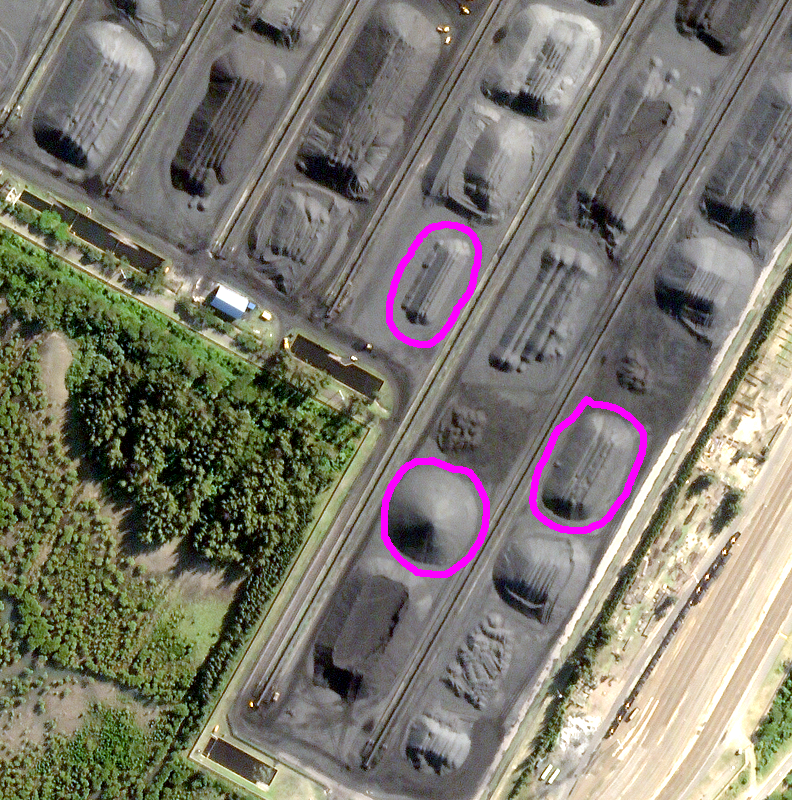
\includegraphics[width=0.48\textwidth]{fs/svi.png}&
	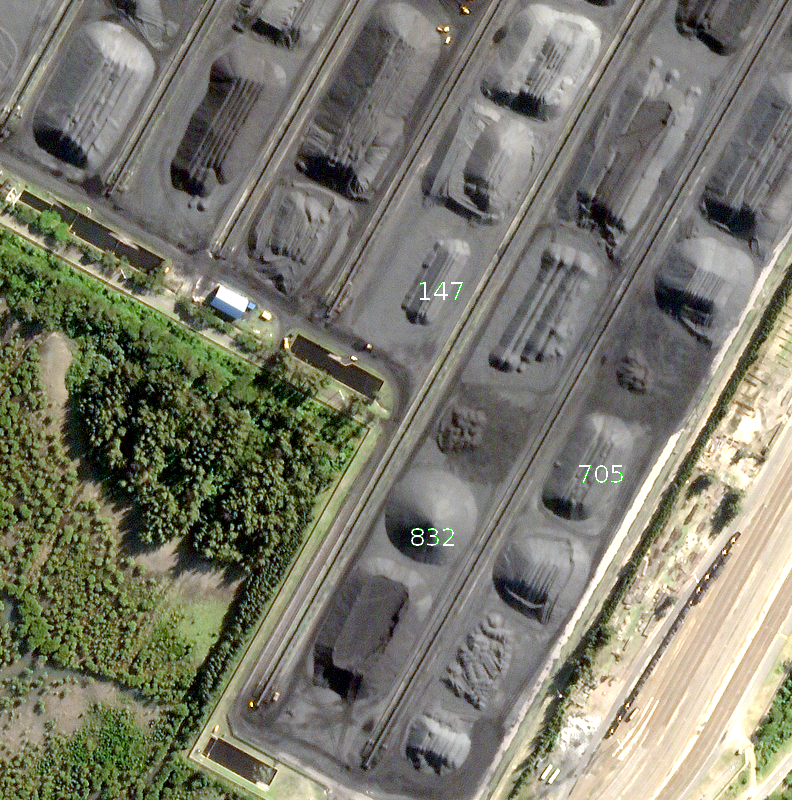
\includegraphics[width=0.48\textwidth]{fs/svo.png}\\
	input &
	output
\end{tabular}
\end{frame}

\begin{frame}
\tt
$ $\\
EXAMPLE\\
=======\\
	\vfill
	\begin{tabular}{cc}
		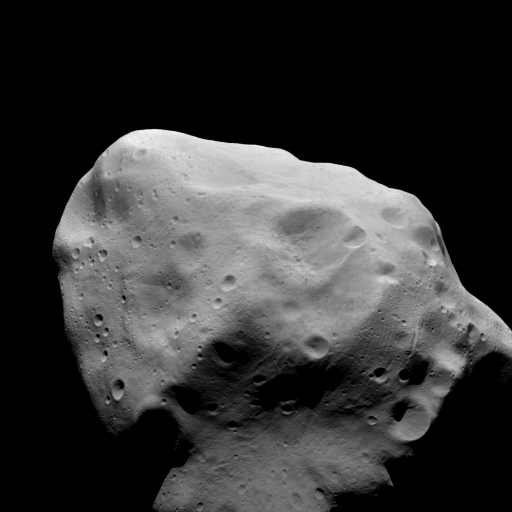
\includegraphics[height=0.4\textwidth]{f/lute_ar.png} &
		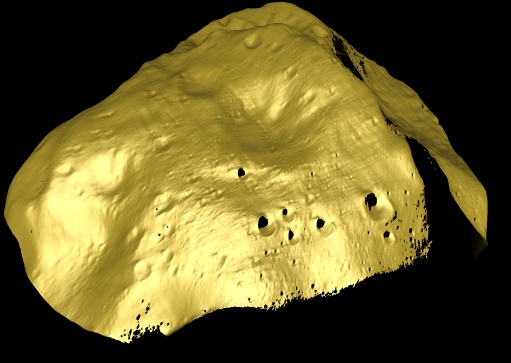
\includegraphics[height=0.4\textwidth]{f/lute_ss.png} \\
		Input (image) & Output (3d model) \\
	\end{tabular}
	\vfill
	\color{gray}ESA Rosetta image of asteroid 21/Lutetia
\end{frame}

\begin{frame}[fragile]
\begin{verbatim}
ALGORITHM
=========


1. Estimate the shape of the coal pile

  1.1. State the lambertian shading equation     A=... b=I
  1.2. Compute viscosity solution           u=(A+eps*L)\b
  1.3. Calibrate parameters                      u=alpha*u

2. Compute the volume of this shape       V=beta*sum(u(:))
\end{verbatim}
\end{frame}

\begin{frame}
\tt
$ $\\
BIBLIOGRAPHY\\
============\\
$ $\\
- B. K. P. Horn\\
 {\it Shape from Shading: a Method for Obtaining the Shape of a Smooth Opaque
	Object from One View }\\
 {\color{gray}
 MIT Technical Report, 1970}

$ $\\
- E. Rouy, A. Tourin\\
  {\it A Viscosity Solutions Approach to Shape-From-Shading }\\
  {\color{gray}
	SIAM J. Numer. Anal, 1992 }

$ $\\
- J.M. Mirebeau, J. Portegies.\\
  {\it Hamiltonian Fast Marching: A Numerical Solver for
  Anisotropic and Non-Holonomic Eikonal PDEs}\\
  {\color{gray} Image Processing On Line 2019}

%$ $\\
%-Z. Chen, Q. Qin,  L. Lin, Q. Liu, Z. Qiong; W. Zhan\\
%	{\it DEM Densification Using Perspective Shape From Shading Through Multispectral Imagery}\\
%	{\color{gray} IEEE Geoscience and Remote Sensing Letters, 2013}


\end{frame}

\begin{frame}
\tt
$ $\\
LIGHTING MODELS\\
===============\\
$ $\\
Lighting of a surface element:
\[
	I=\mathrm{ambient} + (\mathrm{lambertian} + \mathrm{specular})\times \mathrm{binary}
\]
$ $\\
\begin{tabular}{ll}
	ambient& ${\color{red}\alpha\ \times}$ solid angle of visible sky\\
lambertian& ${\color{red}\alpha\ \times}\ \vec n\cdot\vec s$\\
	specular& ${\color{red}\beta\ \times}\ \delta_{{\color{red}\epsilon}}\left(\left\|\vec n-\frac{\vec s+\vec v}{\|\vec s+\vec v\|}\right\|\right)$\\
binary & whether the light source is visible or not \\
& \\
	$\vec n$ & surface normal \\
	$\vec s$ & direction of the light source \\
	$\vec v$ & direction of the point of view \\
\end{tabular}
\end{frame}

\begin{frame}
\tt
$ $\\
LAMBERTIAN MODEL\\
================\\
$ $\\
The lambertian model
\[
	I={\color{lightgray}\alpha}\ \vec n\cdot\vec s
\]
For a surface $z=u(x,y)$ and~$\vec s=(a,b,c)$, this gives
\[
	I = \frac{au_x + bu_y + c}{\sqrt{u_x^2+u_y^2+1}}
\]
which is a first-order PDE that we can solve for~$u$ given boundary conditions.

\vfill
\pause
\fbox{\bf\color{red}WARNING: no solution in the classical sense}
\end{frame}

\begin{frame}
\tt
$ $\\
VISCOSITY SOLUTIONS (EXAMPLE)\\
=============================\\

Some first-order equations have no classical solution:
\[
	\begin{cases}
		\left|u'(x)\right| = 1 & x\in[-1,1] \\
		u(x) = 1 & x\in\{-1,1\}\\
	\end{cases}
\]

\pause
Even solutions ``almost everywhere'' are non unique:
\[
	u_1(x) = |x|\pause
	\qquad
	u_2(x) = 2-|x|\pause
	\qquad
	u_3(x) = \left|x-\tfrac12\right|+\left|x+\tfrac12\right|-|x|
\]
\pause
{\color{blue}Trick:} consider the easier, linear second-order equation
\[
	\begin{cases}
		\left|u'(x)\right| {\color{blue}+\varepsilon u''(x)} = 1 & x\in[-1,1] \\
		u(x) = 1 & x\in\{-1,1\}\\
	\end{cases}
\]
\color{blue} and make~$\varepsilon\to 0$
\end{frame}


%\begin{frame}
%\tt
%$ $\\
%LINEARIZED LAMBERTIAN MODEL\\
%===========================\\
%$ $\\
%In the Lambertian model
%\[
%	I = \frac{au_x + bu_y + c}{\sqrt{u_x^2+u_y^2+1}}
%\]
%we assume~$\sqrt{u_x^2+u_y^2+1}\approx 1$, thus
%\[
%	I = au_x + bu_y + c
%\]
%which is a linear equation (solvable by Matlab's antislash)
%\end{frame}

%\begin{frame}
%\tt
%$ $\\
%LINEARIZED LAMBERTIAN MODEL 2/3\\
%===============================\\
%$ $\\
%The linearized Lambertian model \emph{with  weights} is
%\[
%	I = {\color{blue}w}\cdot(au_x + bu_y + c)
%\]
%where~$w$ depends on $(x,y)$, but not on~$u$.\\
%This model is still linear, and easily solvable.
%
%\vfill
%
%By iteratively re-weighting with~$\color{blue}w=\frac{1}{\sqrt{u_x^2+u_y^2+1}}$,
%we attain a fixed point, which is a solution of the non-linear model.
%
%\end{frame}
%
%\begin{frame}
%\tt
%$ $\\
%LINEARIZED LAMBERTIAN MODEL 3/3\\
%===============================\\
%$ $\\
%This first-order equation is ill behaved:
%\[
%	au_x + bu_y + c - I = 0
%\]
%(1) a solution in the classical sense may not exist, due to incompatible
%boundary conditions\\
%(2) numerically, the solution is independent along each characteristic line,
%leading to artifacts\\
%\vfill
%\pause
%In the spirit of viscosity solutions, we solve instead the well-behaved second order equation
%\[
%	{\color{blue}\epsilon\Delta u}+au_x + bu_y + c - I = 0
%\]
%\end{frame}



\begin{frame}[fragile]
\tt
$ $\\
CODE\\
====\\
$ $\\
	\begin{small}
\begin{minted}{matlab}
	% set up the input data
	M = ...                % mask for the region of interest
	I = ...                % observed gray-scale image
	S = ...                % sun direction field (typically constant)
	epsilon = 0.01         % smoothing parameter

	% set-up the system
	B = grid_graph(I);     % incidence matrix of the whole domain
	C = abs(B)/2;          % centering matrix
	P = C'*diag(S)*B;      % gradient inside the ROI
	P = P - epsilon*B'*B;  % regularization term
	A = M*P + (1-M);       % matrix of the whole system
	b = I;                 % independent term

	% solve the system
	u = A \ b;
\end{minted}
	\end{small}

\end{frame}



\begin{frame}[fragile]
\tt
$ $\\
EXAMPLE\\
=======\\

\begin{tabular}{ll}
	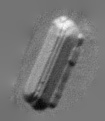
\includegraphics[width=0.2\textwidth]{m/fimcs0.png}&%
\only<1>{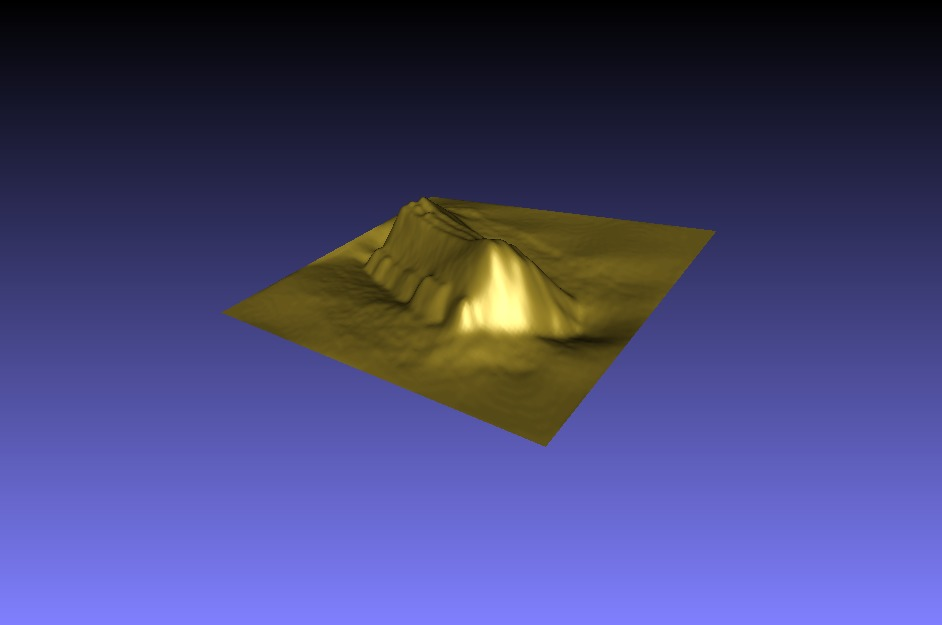
\includegraphics[width=0.8\textwidth]{m/snapshot00.jpg}}%
\only<2>{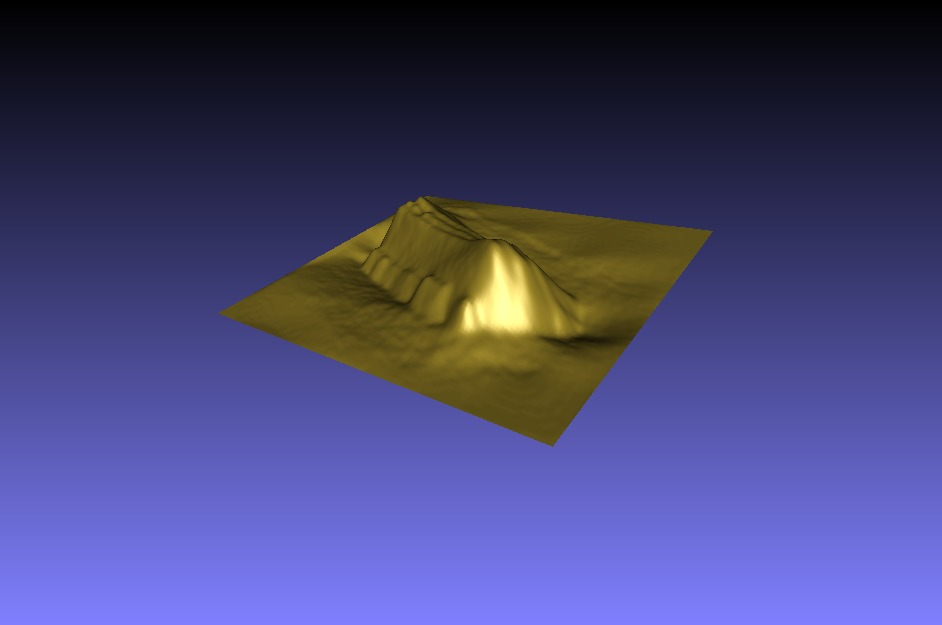
\includegraphics[width=0.8\textwidth]{m/snapshot01.jpg}}%
\only<3>{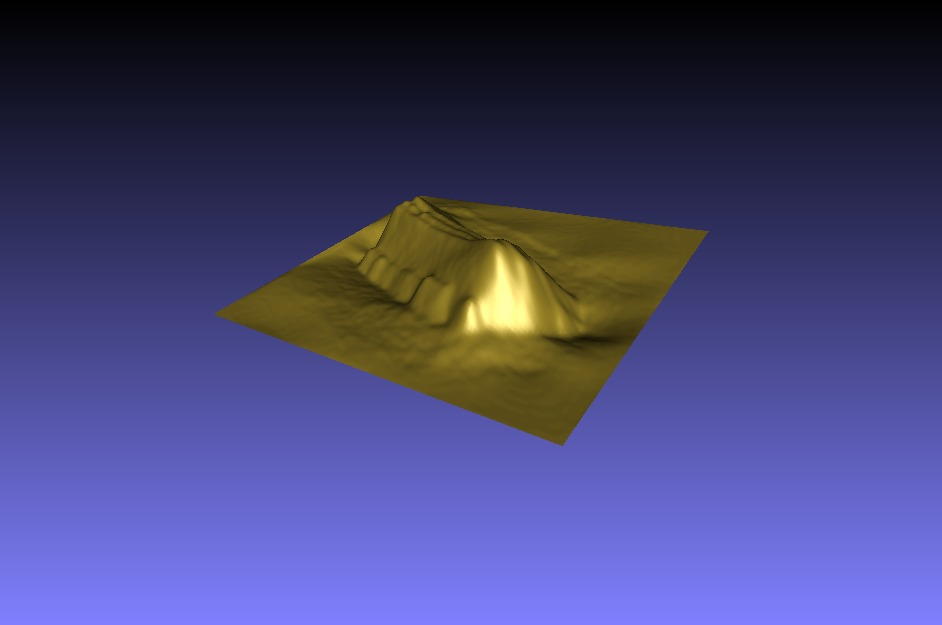
\includegraphics[width=0.8\textwidth]{m/snapshot02.jpg}}%
\only<4>{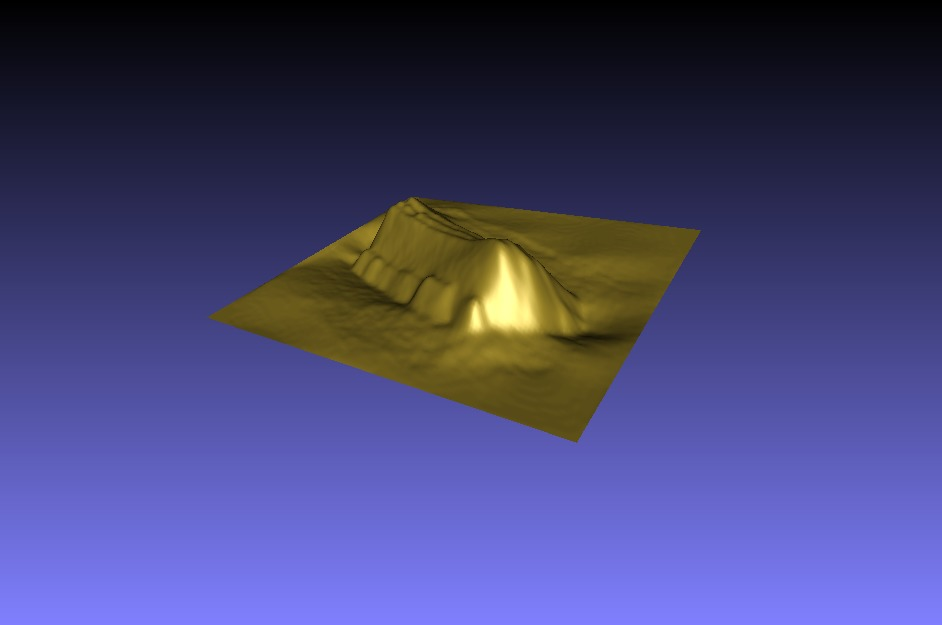
\includegraphics[width=0.8\textwidth]{m/snapshot03.jpg}}%
\only<5>{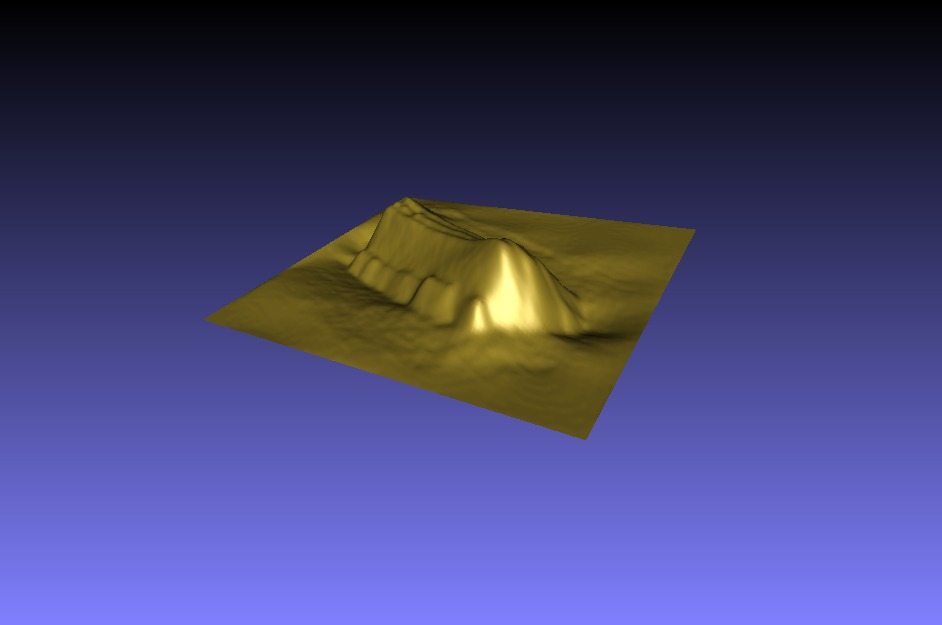
\includegraphics[width=0.8\textwidth]{m/snapshot04.jpg}}%
\only<6>{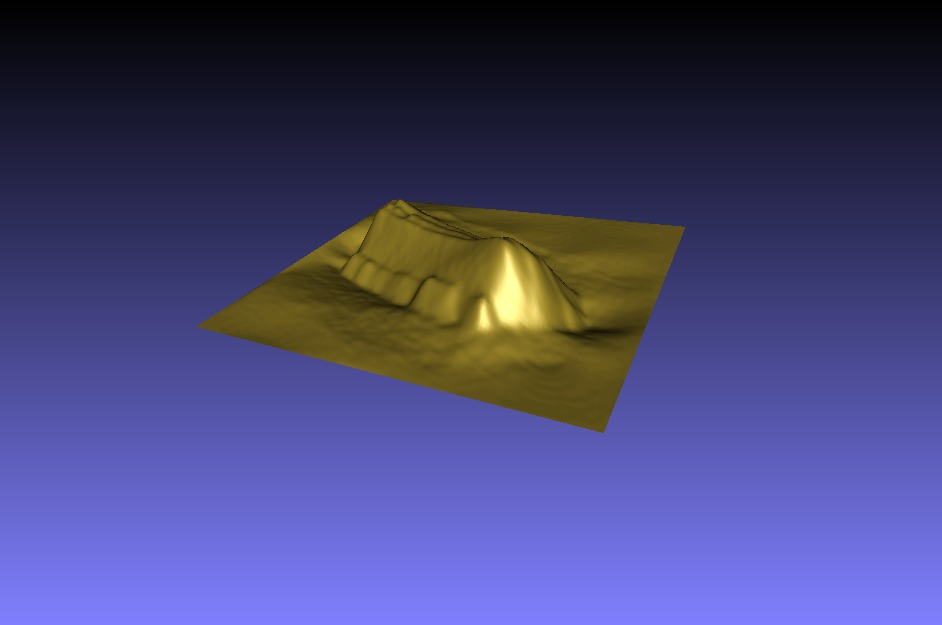
\includegraphics[width=0.8\textwidth]{m/snapshot05.jpg}}%
\\
	\tiny manual selection &
	\tiny output
\end{tabular}
\end{frame}

%\begin{frame}
%\tt
%$ $\\
%EXAMPLE\\
%=======\\
%	\vfill
%	\begin{tabular}{cc}
%		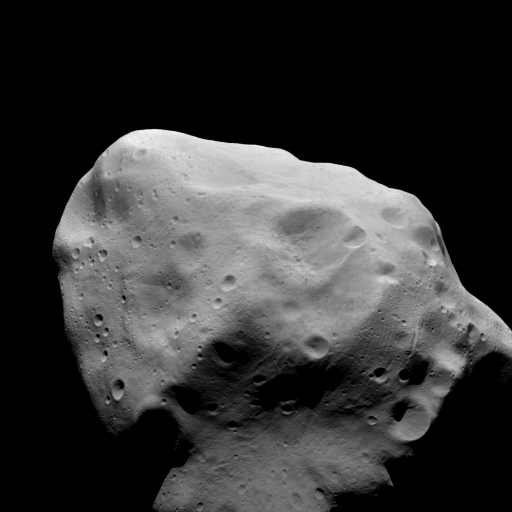
\includegraphics[height=0.4\textwidth]{f/lute_ar.png} &
%		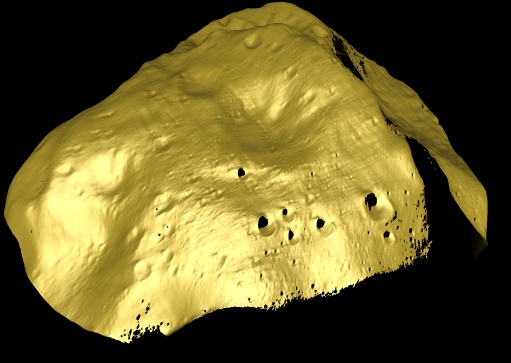
\includegraphics[height=0.4\textwidth]{f/lute_ss.png} \\
%		Input (image) & Output (3d model) \\
%	\end{tabular}
%	\vfill
%	\color{gray}ESA Rosetta image of asteroid 21/Lutetia
%\end{frame}



\begin{frame}[fragile]
\begin{verbatim}
PROGRAMME DU STAGE
==================

1. Maitriser la définition de solution de viscosité
en ``shape from shading''

2. Adapter l'algorithme de Jean-Marie Mirebeau:
2.1. Simplification: domaine isotropique
2.2. Ampliation: conditions de bord mixtes
2.3. Ampliation: régularisation

3. Appliquer la méthode à images réelles:
3.1. Tas de charbon
3.2. Asteroïdes

4. Fournir une implementation en ligne (IPOL)
\end{verbatim}
\end{frame}



\end{document}


% vim:sw=4 ts=4 spell spelllang=en:
